% +------------------------------------------------------------------------+
% | CGAL Reference Manual:  qt_widget.tex
% +------------------------------------------------------------------------+
% | Using Qt_widget to visualize CGAL Objects
% | 
% |
% |
% | 12.12.2001  Radu Ursu
% | 
\RCSdef{\qtwidgetRev}{$Revision$}
\RCSdefDate{\qtwidgetDate}{$Date$}
% +------------------------------------------------------------------------+

\newcommand{\qt}{{\em Qt}}      %QT abbreviation

\gdef\lciIfHtmlClassLinks{\lcFalse}
\gdef\lciIfHtmlRefLinks{\lcFalse}
\gdef\lciIfHtmlLinks{\lcFalse}

\chapter{Qt\_widget}
\label{chapterQtwidget}

\ccChapterRelease{\qtwidgetRev. \ \qtwidgetDate}\\
\ccChapterAuthor{Radu Ursu}

\qt\ is a {\sc Gui} toolkit\footnote{http://www.trolltech.com} for
cross-platform application development. 

% +-----------------------------------------------------+
\section{Introduction}

In this chapter we describe a widget and some helper classes that
allow to interact with two dimensional \cgal\ objects in \qt\ based applications.

The most important class is the class \ccStyle{Qt_widget}. It provides
a drawing area and output stream operators for \cgal\ objects, as well
as zooming and panning functionality.

The \ccStyle{Qt_widget} allows to attach {\em views}, and
it are usually views that draw on the drawing area of the widget.
Views can be activated and deactivated, and what you see in the drawing area
is the overlay of all attached activated views.

The \ccStyle{Qt_widget} allows further to attach one {\em tool} at the time. 
Tools are used for entering input, and \cgal\ provides input tools for the
two-dimensional \cgal\ objects. The limitation to one tool at the time comes
from the fact that only one logical entitiy should get the focus.

Finally, we provide a {\em toolbar} for controlling the basic functionality
of the \ccStyle{Qt_widget}.

The following sections desribe the main class as well as the helper classes
in more detail and give examples that can be taken as starting points for
new applications.


\section{Qt\_widget}
\label{Qt_widget}

The class \ccStyle{Qt_widget} is derived from the \qt\ class \ccStyle{QWidget}%
\footnote{A widget is the atom of the user interface: It receives mouse, keyboard and other 
events from the window system, and paints a representation of itself on the 
screen. Every widget is rectangular, and they are sorted in a Z-order. A 
widget is clipped by its parent and by the widgets in front of it.} 
which is the base class of all \qt\ user interface objects. 


The \ccStyle{Qt_widget} provides output operators for all \cgal\ objects. There are 
operators defined for outputing : points, segments, rays, circles, triangles, 
polygons, and all type of triangulations. Also some operators are defined to 
set \ccStyle{Qt_widget}'s properties, like background and fill color, as well as line
width and point size.

As the following examples show, simple applications can be written
without the views and tools.

\subsection{Example: Hello Segment}
The first example draws a red segment on an orange background.
\ccIncludeExampleCode{../../../test/hellosegment.C}
There is a limitation in this example, you cannot resize the window and keep the drawing.

\subsection{Example: Using Qt\_widget as a stream}

In this example you can see how can you use \ccStyle{Qt\_widget} like a stream, for outputing Cgal objects.

\ccIncludeExampleCode{../../../demo/Qt_widget/basic/tutorial1/tutorial1.C}

In this example as you see, you can use \ccStyle{Qt\_widget} like a stream for output \cgal\ objects.
 There are some limitations in this example. When you resize the window, you will notice that what you have drawn will no longer be there. Like all
the others window applications the code for drawing must be in a redraw function, in order
to work when you will make modifications on the window. In the next example you will see what you have to do to resolve this problem.

\subsection{Example: A Triangulation}

This example is slightly more involved. The user can enter points and the application
draws the Delaunay triangulation of the point set. 

\ccIncludeExampleCode{../../../demo/Qt_widget/basic/tutorial2/tutorial2.C}

Because the code for drawing the triangulation is put in the \ccStyle{redraw()} function, it is drawn after e.g., resize operations. Note that this function first calls \ccStyle{Qt\_widget::redraw()}. It is explained later why this must be done.

\section{Views}
\label{Qt_widget_views}

In the examples from the previous section the code for drawing on the
widget was in the \ccStyle{redraw()} function. As soon as the applications are more 
involved it is better to delegate the drawing task to {\em views}. 
For example, if the application displays a Delaunay triangulation, the corresponding Voronoi diagram,
 and the nearest vertex to the mouse coordinates, it makes
sense to have three independent views. The great advantage of views is that you
 can decide what views you want to see at the runtime, and the other great 
advantage is that views can be reused.

A view can be attached to a \ccc{Qt_widget}. The widget calls the method \ccc{Qt_widget_view::draw()} of all attached views, in the order 
that they were attached. It is a very simple rule, the last view attached will be on top.

Also the views can be activated and deactivated. For example if you have several views attached and you
will deactivate a view, that view will not be drawn anymore on the screen. But when you activate 
the view once again, the view will be placed in the same spot that was before have been deactivated.

By default a view is active when you attach it.

\cgal\ provides some predefined view classes as well as a base class
so that you can more easily write new views.


\subsection{Example: Using A View for Output}
\ccIncludeExampleCode{../../../demo/Qt_widget/basic/tutorial3/tutorial3.C}

As you see, this example is very similar to the previous one, but
the code for drawing the triangulation is no longer in the \ccStyle{redraw()}
 function, instead it is used in a \ccStyle{view}.

This example defines a class derived from \ccStyle{Qt\_widget\_view}. In the member
function \ccStyle{draw()} it is the code for drawing the triangulation. In 
\ccStyle{My\_Window} class you need an instance of \ccStyle{My\_View} and you will have to attach it, if you want to see what the view draws on the screen.

Try to remove the line \ccStyle{attach(&v);} from the constructor to see
what happens. The application will no longer display anything. Try to
deactivate and activate the \ccStyle{view} to see what happens.


\section{Tools}
\label{Qt_widget_tools}

A tool for \ccStyle{Qt_widget} is a class that receives events from
\ccStyle{Qt_widget} and can provide some functionality like input
objects for \ccStyle{Qt_widget} and modify already created
objects. Also some basic operations can be provided like zooming in
and out, or panning.

\cgal\ provides some predefined input tools as well as a convenience base class 
\ccStyle{Qt_widget_tool} for making it easier to develop new tools.

Only one tool at the time can be attached to a widget.

We first show how to use tools and then how they work.

\subsection{Example}

In the previous section, you could insert new points in the triangulation by clicking on the widget. There is another way of doing it. That is where the \ccc{tools} come in. We attach the predefined tool \ccc{Qt_widget_get_point} to the widget, and connect the signal emitted by the widget to the function that 
handles the input.  When the user clicks with the left mouse button, the tool creates
a point and passes it to the widget. The widget then creates a signal that gets passed
to the connected slot \ccc{My_Window::get_new_object(CGAL::Object)}.

\ccIncludeExampleCode{../../../test/tool.C}

The \ccStyle{Qt_widget} forwards all event callbacks to the attached tool.


\subsection{How Tools Work}

The following is an example of a tool that creates \cgal\ points when the user 
clicks the left mouse button over the widget. 
 
\begin{ccExampleCode}
namespace CGAL {

template <class R>
class Qt_widget_get_point : public Qt_widget_tool
{
public:
  typedef typename R::Point_2   Point;
  typedef typename R::FT        FT;
  
  Qt_widget_get_point(const QCursor c=QCursor(Qt::crossCursor)) :
    cursor(c) {};
  
private:
  void mousePressEvent(QMouseEvent *e)
  {
    if(e->button() == CGAL_QT_WIDGET_GET_POINT_BUTTON)
    {
      FT
        x=static_cast<FT>(widget->x_real(e->x())),
        y=static_cast<FT>(widget->y_real(e->y()));
      widget->new_object(make_object(Point(x, y)));
    }
  };
  void attaching()
  {
    oldcursor = widget->cursor();
    widget->setCursor(cursor);
  };
  
  // This function will be called immediately before detaching
  // the tool. The tool is responsible for cleaing up.
  void detaching()
  {
    widget->setCursor(oldcursor);
  };

  QCursor cursor;
}//endclass;
}//namespace CGAL
\end{ccExampleCode}

The \ccc{Qt_widget} forwards mouse and keyboard events to the attached tool.
In the above example only the \ccc{mousePressEvent} member function is overloaded.

Tools that create new \cgal\ objects, must call the member 
function \ccStyle{Qt_widget::new_object(CGAL::Object)}. The \ccStyle{Qt_widget} 
then emits the signal \ccStyle{new_cgal_object(CGAL::Object)}. This signal can be 
catched by any other object with the following connect statement:


connect(Qt\_widget\footnote{This means a pointer to an instance of Qt\_widget},SIGNAL(new\_cgal\_object(CGAL::Object)), anyOtherObject,SLOT(anyOtherFunction(CGAL::Object)));


In the example we connect it to \ccc{MyWindow::get_new_object(CGAL::Object)}.

\section{The Standard Toolbar}
\label{Qt_widget_standard_toolbar}

The standard toolbar includes the basic tools used for zooming and translating.
It's very easy to use, we provide further down a typical model of how to use 
the standard toolbar in your application.

\begin{ccTexOnly}
\begin{center}
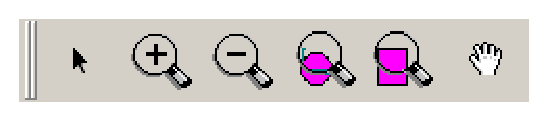
\includegraphics{standard_toolbar.eps} 
\end{center}
\end{ccTexOnly}
\begin{ccHtmlOnly}
<img border=0 src="./standard_toolbar.gif"  align=center  alt="The standard toolbar">
\end{ccHtmlOnly}

\newcounter{bean}
The functionality of the toolbar is like this from the left to right:
\begin{list}
	{Button---\Roman{bean}}{\usecounter{bean}\setlength{\rightmargin}{\leftmargin}}
	\item Remove tool

	\item Zoom In: The scales are multiplied by two keeping the same center

	\item Zoom Out: The scales are divided by two keeping the same center

	\item Zoom In Region: Let you choose the center of the region where you want to zoom in. The scales are multiplied by two

	\item Focus on the Region: The area in the rectangle that you selected will be magnified to best fit in the window.

	\item Hand Tool: Used for translate. Click to select the first point of translation and drag to select the second point.
\end{list}

You can select a tool by clicking on a button of the standard toolbar. To deselect the tool either you press once again the button either you press the arrow button that deselects the active tool, no matter what tool it is.

\ccExample
\ccIncludeExampleCode{../../../test/standard_toolbar.C}

This example generates 100 points and inserts in a delaunay triangulation. Using the standard toolbar you can zoomIn, zoomOut, translate.

\section{The predefined icons}
\label{The predefined icons}
There are some icons defined in some header files. This icons are pixmaps, having the extension .xpm. All the icons are enumerated right here:

\ccInclude{CGAL/IO/pixmaps/arrow.xpm}

\ccInclude{CGAL/IO/pixmaps/hand.xpm}

\ccInclude{CGAL/IO/pixmaps/holddown.xpm}

\ccInclude{CGAL/IO/pixmaps/mouse_coord.xpm}

\ccInclude{CGAL/IO/pixmaps/point.xpm}

\ccInclude{CGAL/IO/pixmaps/line.xpm}

\ccInclude{CGAL/IO/pixmaps/points.xpm}

\ccInclude{CGAL/IO/pixmaps/no_tool.xpm}

\ccInclude{CGAL/IO/pixmaps/zoom_in.xpm}

\ccInclude{CGAL/IO/pixmaps/zoom_out.xpm}

\ccInclude{CGAL/IO/pixmaps/movepoint.xpm}

\ccInclude{CGAL/IO/pixmaps/voronoi.xpm}

\ccInclude{CGAL/IO/pixmaps/triangulation.xpm}

\ccInclude{CGAL/IO/pixmaps/polygon.xpm}

To use a pixmap in your code you have to include the right file, and to know the names of the pixmaps. The names of the pixmaps are composed of two parts, the name of the file and the tag xpm. So for example the arrow pixmap has the name \ccStyle{arrow\_xpm}, the line pixmap has the name \ccStyle{line\_xpm}, and so on \ldots.
In the tutorials and demos, almost all the pixmaps are used for the toolbar buttons, like this:

\ccExample
\begin{ccExampleCode}
    QToolButton *get_point_but;	//the toolbar button
    get_point_but =  new QToolButton(QPixmap( (const char**)point_xpm ),
                                     "Point Tool", 
                                     0, 
                                     this, 
                                     SLOT(pointtool()), 
                                     tools_toolbar, 
                                     "Point Tool");
\end{ccExampleCode}

% +-----------------------------------------------------+
% EOF







